\chapter{Nutrition}

\section*{Number of children under five, women (of childbearing age) and adolescent girls reached by DFID through nutrition-related interventions.}
% make sure numbers and header don't appear
\thispagestyle{empty}

\section{Results}

From 2015-2020 DFID reached \textbf{55.1 million} children under 5, women of childbearing age and adolescent girls through our nutrition-relevant programmes. %

\begin{figure}[htbp]
	\centering
	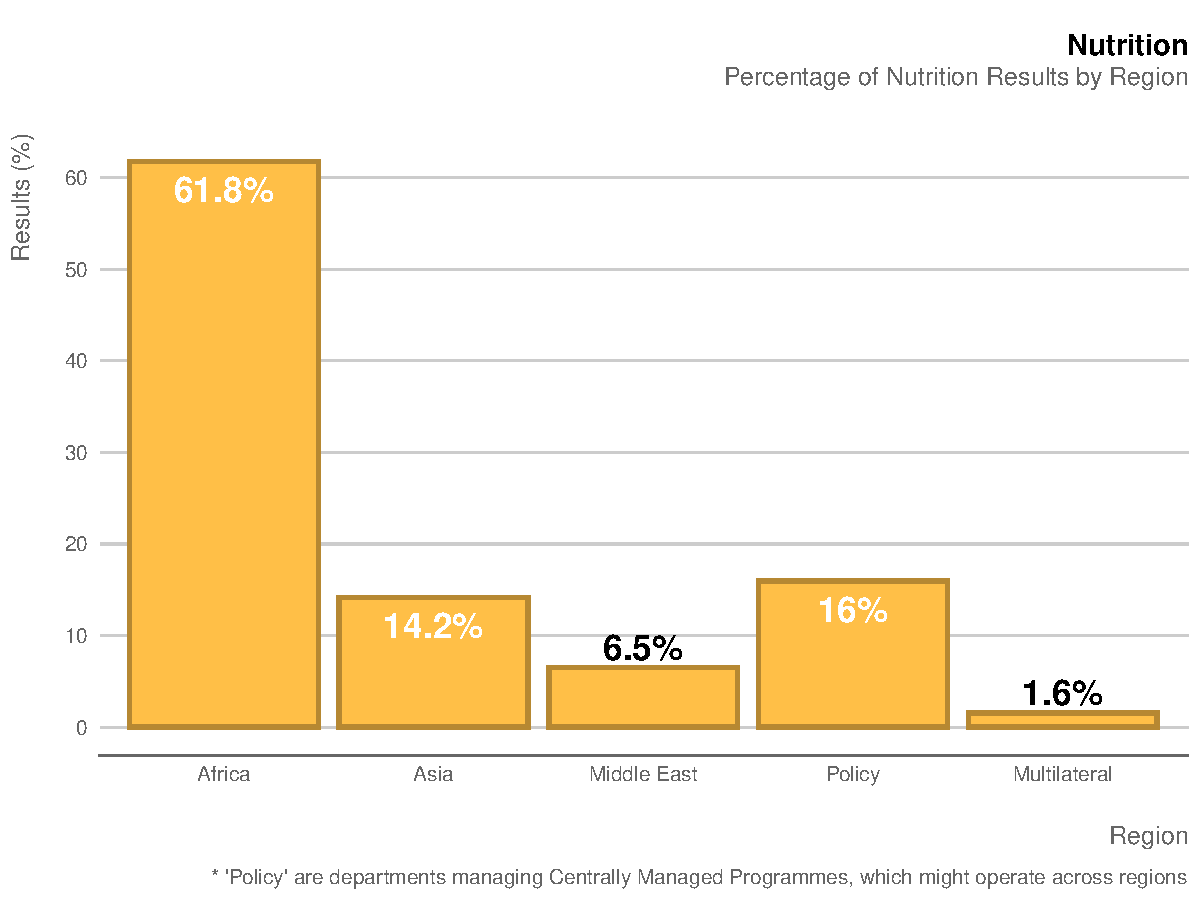
\includegraphics[width=0.8\textwidth]{../figs/nutrition_region_plot} \hfill
	\caption{Percentage of Nutrition results by region.}\label{fig:nutrition_region_plot}
\end{figure}


From 2015 to 2020, Africa was the largest beneficiary of DFID’s nutrition-related programmes, with 37.5 million beneficiaries reached (see Figure \ref{fig:nutrition_region_plot} for regional percentage breakdown). %
DFID reached 8.6 million beneficiaries in Asia: the majority of whom were in Bangladesh (6.1 million). %
DFID reached 3.9 million beneficiaries in the Middle East: the majority of whom were in Yemen (3.5 million). %
A further 10.6 million beneficiaries of DFID's nutrition results were delivered via non-country or -region specific programmes, and multilateral organisations. %

Most of the children under 5, women of childbearing age and adolescent girls (48.4 million beneficiaries) reached by DFID’s nutrition-related programmes live in fragile states (using the OECD States of Fragility definition), including 15.2 million beneficiaries living in Extremely Fragile States (Figure \ref{fig:nutrition_fragility_plot}). %

\begin{figure}[htbp]
	\centering
	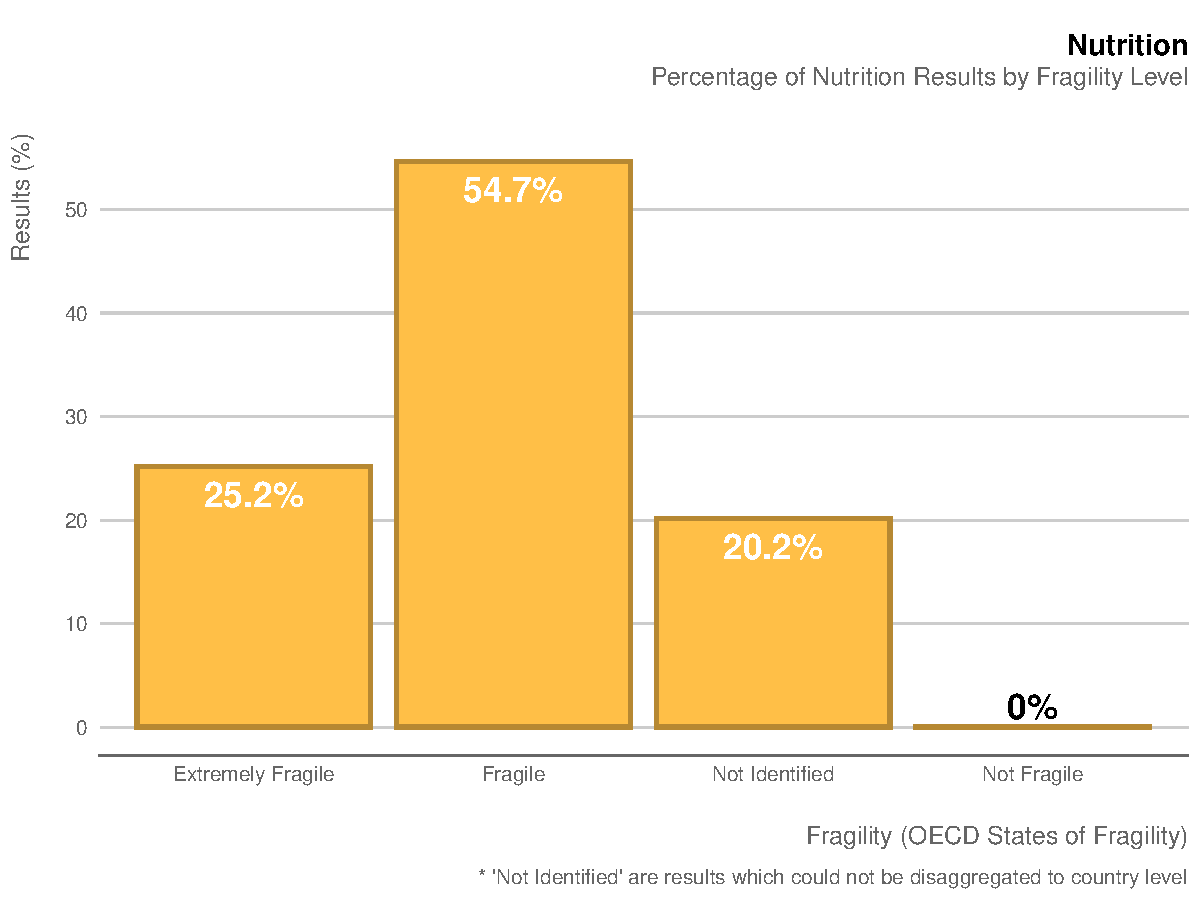
\includegraphics[width=0.8\textwidth]{../figs/nutrition_fragility_plot} \hfill
	\caption{Percentage of Nutrition results by fragility level.}\label{fig:nutrition_fragility_plot}
\end{figure}


High, medium and low intensity results are defined according to:
\begin{itemize}
	\item Comprehensiveness of the package reaching the target population
	\item Whether this package is directly or indirectly targeted to this target population
\end{itemize}

In all cases, `target population' refers to women of childbearing age (15 to 49 years), children under 5 years and adolescent girls (10 to 19 years). %
Please refer to the methodology summary, and the published methodology note for more details. %

\begin{figure}[htbp]
	\centering
	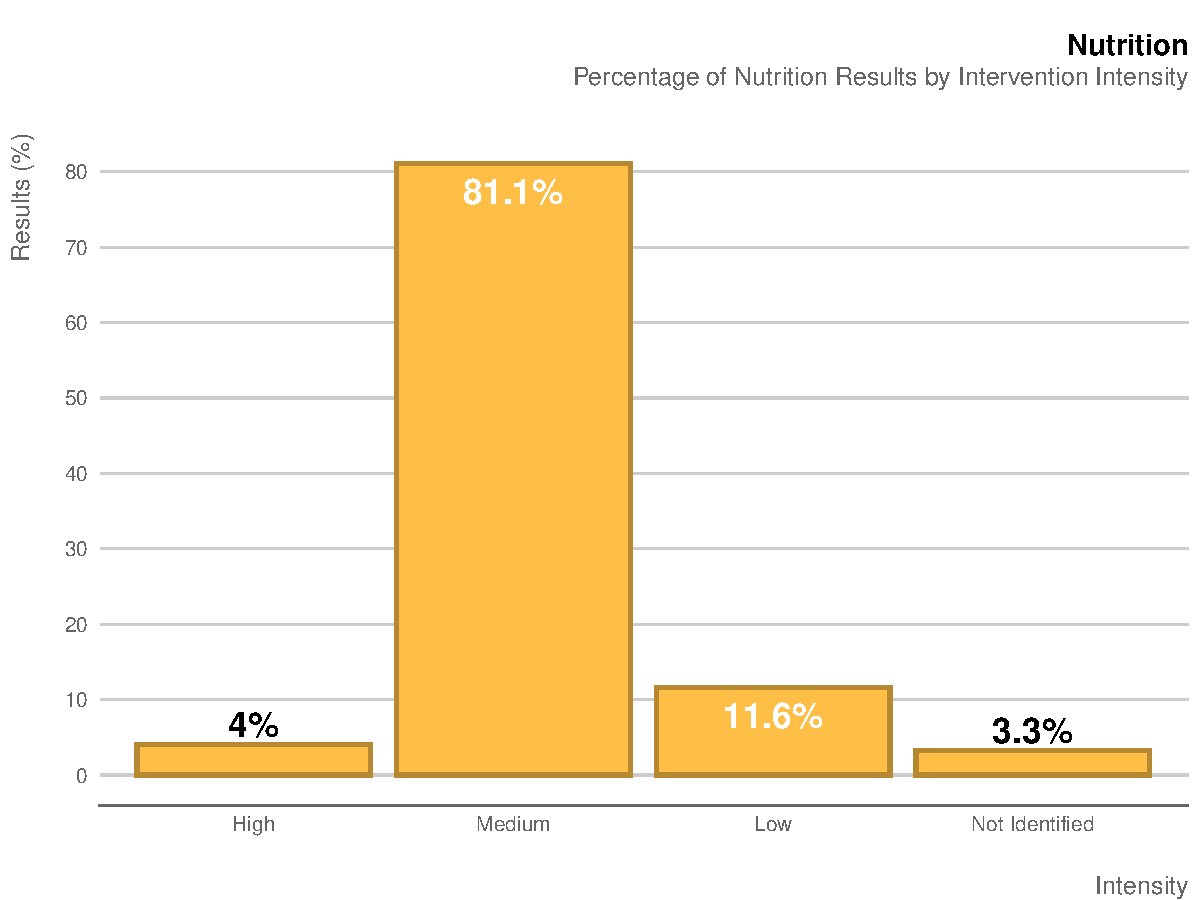
\includegraphics[width=0.8\textwidth]{../figs/nutrition_intensity_plot} \hfill
	\caption{Percentage of Nutrition results by intervention intensity.}\label{fig:nutrition_intensity_plot}
\end{figure}

Most of the beneficiaries of DFID nutrition-related programmes received medium intensity intervention (49.9 million beneficiaries; Figure \ref{fig:nutrition_intensity_plot}). %
DFID nutrition-related programmes reached 2.4 million beneficiaries with high intensity intervention and 7.1 million beneficiaries with low intensity interventions. %
Intensity information was not available for 2 million beneficiaries of DFID's nutrition results\footnote{The total number beneficiaries counted from the different intensities of intervention may exceed the overall total number of beneficiaries reached on Page 1.This is due to the application of the peak year method at the country level: the overall total achieved counts the single year with the largest number of results within a country. Since the ``peak'' reach within a country may occur in different years for each intensity level, the total achieved by intensity may sum across different years, resulting in a larger reach than the overall total.}. %

Of those reached by DFID nutrition-related programs from 2015 to 2019, 24 million were women and girls. %
DFID is continuously working with our existing partners towards improving collection of disaggregated data. %
In 2018/19 50\% of our reported nutrition results were disaggregated by gender. %


\section{Context}

Good nutrition plays a key role in child development. Children who are undernourished are more likely to get sick or die. %
Those who survive suffer impaired physical growth and brain development, which limits educational attainment and lifelong earning potential. %
Under-nutrition remains a major challenge in developing countries including those that face humanitarian crises. %

Globally, there are an estimated 144 million children under 5 who are stunted (too short for their age, which can limit brain development) and 47 million who are wasted (low weight for their height, which can increase the risk of death) due to poor nutrition\footnote{UNICEF/WHO/World Bank Group (2020). Joint Child Malnutrition Estimates 2018 edition. New York. Available at: \href{https://data.unicef.org/resources/jme/}{https://data.unicef.org/resources/jme/}}. %
The greatest burden of undernutrition falls within Africa and Asia, with almost one in three children in Africa suffering from stunting, and almost one in four children in Asia. %
Sustainable Development Goal 2 aims to end hunger, achieve food security and improved nutrition and promote sustainable agriculture, and includes a specific target to end all forms of malnutrition by 2030. %
The recent pace of change is insufficient to meet this target, and in some countries no progress or a worsening of the situation has been seen\footnote{Development Initiatives (2017). Global Nutrition Report 2017: Nourishing the SDGs. Bristol: Development Initiatives. Available at: \href{https://www.globalnutritionreport.org/files/2017/11/Report_2017.pdf}{https://www.globalnutritionreport.org/files/2017/11/Report\_2017.pdf}}. %

Interventions to improve nutrition among children, adolescent girls and women of childbearing age can result in a return on investment of \pounds 16 for every \pounds 1 spent\footnote{Hoddinott, J (2016). Global Panel on Agriculture and Food Systems for Nutrition Working Paper: The economics of reducing malnutrition in Sub-Saharan Africa. Available at: \href{http://glopan.org/sites/default/files/Global_Panel_Working_Paper.pdf}{http://glopan.org/sites/default/files/Global\_Panel\_Working\_Paper.pdf}}. %
The 2013 Lancet Commission on Maternal and Child Nutrition recommended the scale-up of a package of ten key interventions to directly address the causes of under-nutrition (the so-called nutrition-specific package), based on the available evidence of efficacy\footnote{Bhutta, Z.A. et al. (2013). Evidence-based interventions for improvement of maternal and child nutrition: what can be done and at what cost? The Lancet, Volume 382, Issue 9890, pp. 452-477}. %
It was estimated that 90\% coverage of these interventions could reduce under-five deaths by 15\%. %
However, scale-up of the nutrition-specific package alone will only address 20\% of the burden of stunting, given the influence of a range of other factors on child stunting. %
To address the remaining 80\% of the stunting burden, cross-sectoral actions (nutrition-sensitive interventions) are required to address the underlying determinants of under-nutrition\footnote{Ruel, M.T. et al. (2013). Nutrition-sensitive interventions and programmes: how can they help to accelerate progress in improving maternal and child nutrition? The Lancet, Volume 382, Issue 9891, pp. 536-551}. %

\newpage
